\documentclass{llncs}

\usepackage{amsmath}
\usepackage{algorithmicx}
\usepackage{algpseudocode}
\usepackage{cite}
\usepackage{flushend}
\usepackage{graphicx}
\usepackage{graphics}
\usepackage{url}
\usepackage[table]{xcolor}
\usepackage{xspace}
\usepackage[T2A]{fontenc}

\usepackage{algorithm}
\usepackage[english]{babel}

\usepackage[utf8]{inputenc}

\newboolean{doubleblind}
\setboolean{doubleblind}{false}

\allowdisplaybreaks

\begin{document}
 We are solving the problem of the bounds on expected runtime of the evolutionary algorithm that generates test for Dijkstra algorithm such that this algorithm will relax all edges during this test.
 
 \section{Experiments}
 
 First we made some experiments that calculated:
 \begin{itemize}
  \item average number of algorithm iterations depending on the number of edges with the fixed number of vertices;
  \item average number of algorithm iterations depending on the number of vertices with the fixed number of edges;
  \item average number of leaves in the generated graph during the algorihm runtime;
  \item average number of vertices in the connected component;
 \end{itemize}
 
 \subsection{Algorithm iterations}
  We made 200 algorithm runs for each number of edges and vertices and counted the number of iterations. For fixed numbers we made experiments with 5, 10 and 15 vertices and 10, 20 and 30 edges. Here are results:
  
  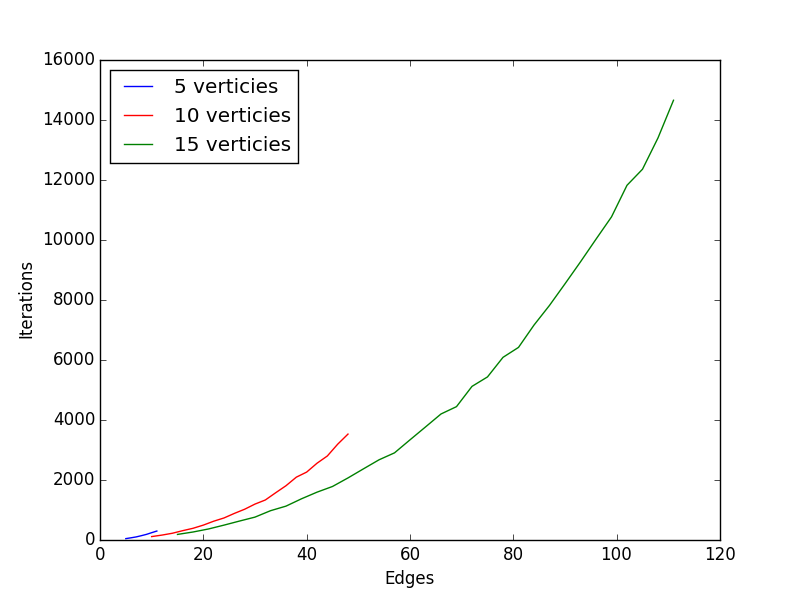
\includegraphics[height=5cm]{pic/const_vertices.png}
  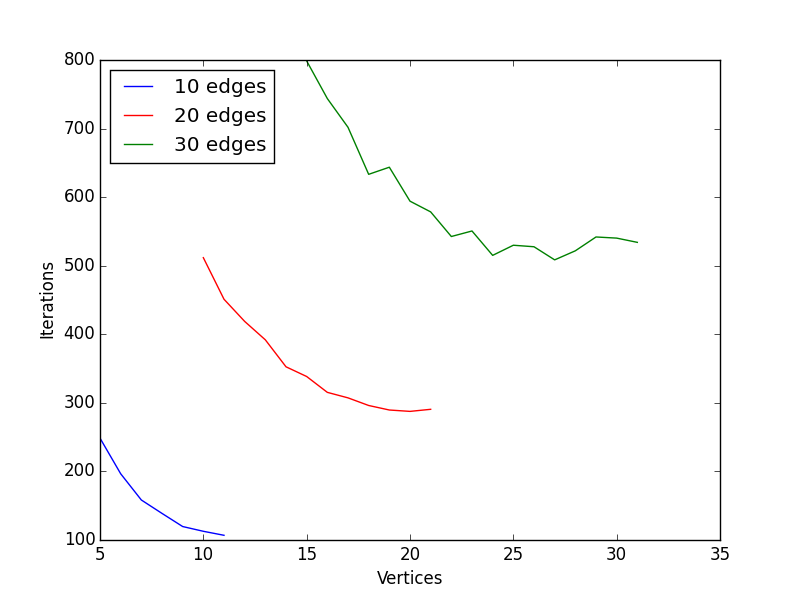
\includegraphics[height=5cm]{pic/const_edges.png}
  
  We can see that expected runtime depends straightly on the number of edges and inversely depends on the number of vertices.
  
 \subsection{First analysis}
  The algorithm run can be divided into two phases:
  \begin{itemize}
   \item the phase of growth, when all the vertices become reacheble from the start one;
   \item the phase of relaxing all edges that left unrelaxed in te first phase.
  \end{itemize}

  The analysis of the first phase is comlex because of two facts:
  \begin{itemize}
   \item in some cases size of connected component decreases by one;
   \item in some cases connected component can be extended by more than one vertex.
  \end{itemize}
  
  But we have an assumption that the first fact doesn't have much influence on the upper bound of the first phase because it's qute rare situation.
  The second fact only decreases the upper bound on runtime of the first phase.
  So we can make simple upper bound on the expectation of runtime of the first phase.
  
  The probability of the extention of the connected component by one vertex is not less then multiplication of probabilities 
  of taking the edge not from the spanning tree on the probability of putting it's new start into the connected component and it's end outside the connected component:
  
  $$P_{inc} \ge \frac{E - i + 1}{E} \cdot \frac{i(V - i)}{V^2},$$
  
  where $E$ -- number of edges, $V$ -- number of vertices in the graph, $i$ -- number of vertices in the current connected component.
  
  
  So the expectation of the extension of the connected component by one vertex is following:
  
  $$E_{inc} = P_{inc}^{-1} = \frac{EV^2}{(E - i + 1)i(V - i)}$$
  
  The expected runtime of the first phase can be calculated as the sum of expected times of extension by one vertex for every size of the connected component:
  
  \begin{align*}
   E_{i=V} & = \sum_{i = 1}^{V - 1} \frac{EV^2}{(E - i + 1)i(V - i)} = \sum_{i = 1}^{V - 1} \frac{EV}{E - i  + 1} \left( \frac{1}{V - i} + \frac{1}{i}\right) = \\
	  & = \sum_{i = 1}^{V - 1} \left( \frac{EV}{E - V + 1} \left( \frac{1}{V - i} - \frac{1}{E - i + 1} \right) + \frac{EV}{E + 1} \left( \frac{1}{i} + \frac{1}{E - i + 1} \right) \right) = \\
	  & = EV \left( \frac{1}{E - V + 1} + \frac{1}{E + 1} \right) \sum_{i = 1}^{V - 1} \frac{1}{i} + EV \left( \frac{1}{E + 1} - \frac{1}{E - V + 1} \right) \sum_{i = 1}^{V - 1} \frac{1}{E - i + 1} \approx \\
	  & \approx \frac{V(2E - V)}{E - V} \ln{V} - \frac{V^2}{E - V} (\ln{E} - \ln{(E - V)} )
  \end{align*}

 
 
\end{document}
